\documentclass[a4paper,reqno]{article}
\addtolength{\textwidth}{2cm} \addtolength{\hoffset}{-1cm}
\addtolength{\textheight}{2cm} \addtolength{\voffset}{-.5cm}
\usepackage{amssymb}
\usepackage{amsmath}
\usepackage{amsthm}
\usepackage{graphicx}
\usepackage{amsfonts}
\usepackage[usenames]{color}
\usepackage{hyperref}
\usepackage{mathtools}
\mathtoolsset{showonlyrefs}
\usepackage{hyperref}
\usepackage[utf8]{inputenc}
\usepackage{listings}
\usepackage{color}


\definecolor{gray}{RGB}{100,100,100}
\definecolor{basiccolor}{RGB}{0, 43, 54}
\definecolor{keywordscolor1}{RGB}{88, 110, 117}
\definecolor{keywordscolor2}{RGB}{101, 123, 131}
\definecolor{keywordscolor3}{RGB}{147, 161, 161}
\definecolor{identifiercolor}{RGB}{37, 116, 206}
\definecolor{commentscolor}{RGB}{91, 69, 0}
\definecolor{attributescolor}{RGB}{203, 75, 22}
\definecolor{numberscolor}{RGB}{147, 161, 161}
\definecolor{stringscolor}{RGB}{48, 145, 134}
\definecolor{backgroundcolor}{RGB}{255, 255,255}

% DEFINE LSTSET

\lstset{basicstyle = \color{basiccolor}\footnotesize\ttfamily,                   % the size of the fonts that are used for the code
  identifierstyle = \color{identifiercolor},
  commentstyle = \itshape\color{commentscolor},            % comment style
  keywordstyle = \bfseries\color{keywordscolor1},          % keyword style
  keywordstyle = {[2]\bfseries\color{keywordscolor2}},
  keywordstyle = {[3]\bfseries\color{keywordscolor3}},
  keywordstyle = {[4]\bfseries\color{attributescolor}},
  stringstyle = \color{stringscolor},                     % string literal style
  backgroundcolor = \color{backgroundcolor},
  inputencoding=utf8,
  extendedchars=true,
  literate=%
        {é}{{\'{e}}}1
        {è}{{\`{e}}}1
        {ê}{{\^{e}}}1
        {ë}{{\¨{e}}}1
        {É}{{\'{E}}}1
        {Ê}{{\^{E}}}1
        {û}{{\^{u}}}1
        {ù}{{\`{u}}}1
        {ú}{{\'{u}}}1
        {â}{{\^{a}}}1
        {à}{{\`{a}}}1
        {á}{{\'{a}}}1
        {ã}{{\~{a}}}1
        {Á}{{\'{A}}}1
        {Â}{{\^{A}}}1
        {Ã}{{\~{A}}}1
        {ç}{{\c{c}}}1
        {Ç}{{\c{C}}}1
        {õ}{{\~{o}}}1
        {ó}{{\'{o}}}1
        {ô}{{\^{o}}}1
        {Õ}{{\~{O}}}1
        {Ó}{{\'{O}}}1
        {Ô}{{\^{O}}}1
        {î}{{\^{i}}}1
        {Î}{{\^{I}}}1
        {í}{{\'{i}}}1
        {Í}{{\~{Í}}}1}


\newcommand{\myenv}{(\raisebox{0pt}{\mygraphic{.6em}})}
\newcommand{\pa}{\hspace{1cm}}

\begin{document}

\title{Projet 2A : La chambre la moins froide}
\author{Tanguy VIVIER, \\
Rémi MOUZAYEK}
\maketitle
\newpage

\setlength{\parindent}{1cm}
\part*{Introduction}
L'équation de la chaleur est une équation aux dérivées partielles 
parabolique, pour décrire le phénomène physique de conduction thermique, introduite initialement en 1811 par Jean Baptiste Joseph Fourier. Cette problématique de la diffusion de la chaleur est un enjeu industriel central vos à vis la gestion de l'énergie. A l'heure de la COP 21, elle n'a d'ailleurs jamais semblée autant d'actualité. \\
Comment maximiser la température d'une chambre en ne jouant que sur la géométrie de cette dernière ? Cette question qui peut surprendre de prime abord - car des dogmes architecturaux nous pousse naïvement à supposer, par définition, que toute chambre respectable se doit d'être rectangulaire - prend alors tout son sens.
Cette recherche se place indéniablement dans un vaste domaine d'étude, au confluent des mathématiques et de l'informatique: l'optimisation de forme. \\


% PARTIE 1 
\part{Mise en place de l'étude}

Notre étude sera réalisée en deux dimensions, dans le plan $\mathbb{R}^2$. Par ailleurs, une chambre sera modélisée par un polygone. Nous allons principalement nous intéresser aux pentagones (polygones à 5 côtés), cependant d'autres polygones seront également testés pour mener à bien ce travail. \\
Cette étude n'est rien d'autre qu'un problème d'optimisation. En effet, nous chercherons à maximiser le critère: température moyenne d'une pièce dans \textbf{son régime stationnaire}. \\ Pour fixer les notations, à l'avenir, la température à la position repérée par le vecteur $x$ de la chambre $\Omega$ au temps $t$ sera notée $u(x,t)$. De plus, la température moyenne de la pièce s'exprime facilement par  $ \frac {1}{|\Omega|}\int_{\Omega} u(x,t) dx $ ou $|\Omega|$ représente l'aire de la chambre.\\
Par ailleurs, nous considérerons que la température dans la pièce $\Omega$ est pilotée par l'équation aux dérivées partielles: 
\\
\begin{equation}
\frac{\partial u}{\partial t}(x,t) = \Delta u(x,t) + f(x,t)
\end{equation}
Il s'agit de l'équation de la chaleur usuelle dans laquelle les diverses constantes caractéristiques du phénomène ont été égalisé à 1. Par ailleurs, $f(x,t)$ est un terme de source permettant de préciser le profil thermique de la pièce.
Une des données clef de ce problème est de bien comprendre que dés lors que nous souhaitons classer des polygones (ou plus généralement des formes géométriques quelconques) il faut nécessairement que nous fixions des caractéristiques. En effet comment comparer la température moyenne de deux pièces si pour un même radiateur elles sont d'aires ou de nombre de cotés différents ? \\
Voici le cahier des charges retenus: \\
- le nombre de sommets du polygone est fixé égal à 5 dans l'étude principale, c'est à dire que nous travaillons sur des pentagones; \\
- l'aire des polygones est fixée égale à $|\Omega|$; \\
- toutes les chambres seront chauffées grâce à un même radiateur. Pour le modéliser, nous considérerons qu'un mur (c'est à dire un coté du polygone) de longueur fixée $l$ est sujet à un flux thermique entrant $\Phi$e connu et, également fixé;  \\
- la chambre est supposée isolée: les températures surfaciques des autres murs (cotés du polygone) sont fixées égales à une même constante $T_{0}$; \\
- Nous considérons un profil thermique identiquement nul : $f(x,t)  = 0$.
\\
Le problème est désormais bien posé. Il faut cependant garder à l'esprit que les contraintes fixées ici sont fortes: voyager à aire constant avec la position de deux sommets données est particulièrement contraignant. Une part importante de l'étude est de réfléchir à l'implémentation d'un algorithme pour pouvoir générer des polygones respectant ces contraintes.


% PARTIE 2
\part{Étude préliminaire: le cas des triangles}
\section*{I - Cadre général de l'étude}
On va considérer le problème simple d'une pièce triangulaire dans toute cette partie. On considère aussi une application $T_S$ qui a une valeur $x$ va associer un triangle d'aire $S$ et de côtés de longueur $x$ et $1$. La fonction $u_\Omega$ correspond à la solution de l'équation précédente sur le domaine $\Omega$, qui est dans le cas ici présent un triangle. On va noter $M$ la fonction qui renvoie la moyenne de $u_\Omega$ sur $\Omega$ telle que $M(\Omega) = \frac {1}{|\Omega|}\int_{\Omega} u_\Omega(x,t) dx $. \\
Désormais, on pose $ F = M\circ T $. Le problème formulé ci-dessus revient donc à chercher le $x$ qui maximise la fonction F, on se ramène ainsi à un problème d'optimisation de $\mathbb{R}$ dans $\mathbb{R}$. \\
\\
Pour étudier le problème dans un premier temps, on va considérer un côté fixe de longueur 1 centré sur l'axe des ordonnées. Ensuite on va faire varier le côté adjacent de longueur $x$. En sachant que l'aire du triangle est fixée, on pourra déterminer le triangle correspondant en fonction du seul paramètre $x$. On note E l'ensemble des sous-ensembles de $\mathbb{R} ^{2}$\\
\vspace{1.5cm}
\begin{center}
\begin{picture} (100,100) (-120,-20) 
\setlength{\unitlength}{2cm}
\thicklines
\put(-4,0.8) {$T_\Omega : \mathbb{R} \longmapsto E$ }
\put(-3.6,0.6){$x \longrightarrow $ Triangle de côté 1 et x, d'aire $|\Omega|$}
\put(0,0) {\line(0,1) {2}}
\put(0,0) {\line(1,0) {2}}
\put(0,2) {\line(1,-1) {2}}
\put(-0.2,0.8) {$1$}
\put(1.1,1.1) {$x$}
\put(0.5,0.7) {$|\Omega|$}
\end{picture}
\end{center}
\vspace{2cm}
Dans la suite de l'étude, on va considérer le côté fixé de longueur 1 sur l'axe des ordonnées, centré sur l'origine (C'est à dire les deux premiers points du triangle en (0, 0.5) et (0, -0.5)). Le dernier point du triangle peut ainsi être déterminé grâce à la seule connaissance de $x$. Par soucis de simplification, on va ainsi poser la fonction $T$ qui renvoie les coordonnées du dernier point en fonction de $x$. Le triangle pourra ainsi être tracé car on connait les deux autres coordonnées. Ce dernier point est de coordonnées : $(2|\Omega|,\frac{1}{2} - x\sqrt{1-(\frac{2|\Omega|}{x})^2})$. (On peut déterminer ces formules à l'aide de calculs simples sur les relations d'Al-Kashi)\\

Sur Matlab, on a implémenté une fonction qui construit un objet de type "geometry" triangulaire en fonction de l'aire $\Omega$ et de la longueur du côté $x$. Cet objet geometry définit la forme de la zone sur laquelle on va rédoudre l'équation différentielle. 

\newpage

\begin{lstlisting}[language=Matlab,frame=single,caption=Construction d'une géométrie Triangulaire]
function g = triangle(X,area)

% TRIANGLE
% Renvoie la geometrie d'un triangle d'aire fixee et de longueurs de cote 
% X et Y 

if (X.^2<0.25)
    g = "Un tel triangle n'existe pas" 
else 
    mat = [2;3;0;0;2*area;-0.5;0.5;0.5-X*(1-(2*area/X)^2)^.5] ; 
    [dl,bt] = decsg(mat) ;
    g = dl ;
end
\end{lstlisting}

%SECTION 2
\section*{II - Première étude : Conditions simples}

On va considérer ici des conditions relativement simples. Premièrement, on se place en régime stationnaire, c'est à dire que le terme $\frac{\partial u}{\partial t}$ est nul. De plus, on fixe une fonction de chauffage nulle. Enfin, les conditions aux limites sont fixées telles que le côté de longueur fixée $1$ soit traversé par un flux positif (modélisant un chauffage), et les deux autre côtés sont fixés à une température extérieure $T_0$ (dans le cas présent fixé à 10).
\vspace{3cm}
\begin{center}
\begin{picture} (100,100) (-10,-10) 
\setlength{\unitlength}{2.5cm}
\thicklines
\put(0,0) {\line(0,1) {2}}
\put(0,0) {\line(1,0) {2}}
\put(0,2) {\line(1,-1) {2}}
\put(-0.1,2.1) {$A$}
\put(2.1,0) {$B$}
\put(-0.2,-0.1) {$C$}
\put(-0.2,1) {$1$}
\put(1.1,1.1) {$x$}
\put(0.7,0.7) {$\Omega$}
\put(-1,0.8) {\vector(1,0){1.3}}
\put(-1,0.65) {$\phi $ : flux entrant}
\put(1.7,1) {Température extérieure fixée $T_0 = 10$}
\end{picture}
\end{center}
En clair les conditions aux limites sont de la forme : 
\begin{equation}
\left\{
	    \begin{array}{ll}

		\mbox{Dirichlet sur }  (AB)\cup (CB)\mbox{:     }u_\Omega=10 \\
		\mbox{Neumann sur } (AC)\mbox{:    }-grad(u_\Omega).n = 50
	    \end{array}
\right.		
\end{equation}
On peut résoudre l'EDP sur l'exemple ci-dessus avec Matlab assez facilement. On prend dans cette résolution la valeur x =$\sqrt{2}$ et $|\Omega| = 1/2$ pour que cela corresponde au dessin ci-dessus. 
\begin{center}
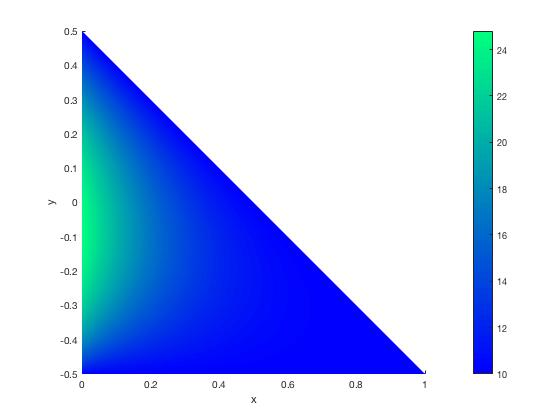
\includegraphics[scale=0.5]{TriangleEDP.jpg}
\end{center}
Voici le script matlab correspondant (Les fonctions seront explicitées ultérieurement) :
\vspace{0.5cm}



% LISTING2 
\begin{lstlisting}[language=Matlab,frame=single,caption=Resolution d'une EDP sur un triangle]
function result = uTriangle(X,area,fc)

model = createpde() ; 
g=triangle(X,area) ; 
% Construit un triangle de cote X et d'aire area
geometryFromEdges(model,g); % geometryFromEdges for 2-D

%Conditions de bord : 
%Les murs non chauffes sont a la temperature exterieure To = 10
applyBoundaryCondition(model,'dirichlet','Edge',[2,3],'u',10);

%Le mur chauffe est modelise par un flux rentrant 
% on suppose que l on a mis un radiateur au niveau du mur 
applyBoundaryCondition(model,'neumann','Edge',[1],'q',0,'g',50);

% Parametres de l'equation
a = 0;
c=1;
a=0;
f=fc;
% On choisit une maille adaptative, car les coins du triangle sont un probleme
[u,p,e,t] = adaptmesh(g,model,c,a,f,'maxt',5000,'par',1e-10);
pdeplot(p,e,t,'XYData',u,'ZData',u,'Mesh','off')
xlabel('x')
ylabel('y')
xlim([-X X])
ylim([-X X])
axis equal
result.u = u ;  % Valeur de u sur chaque mesh
result.p = p ;  % Coordonnees des points 
result.t = t ;
result.e = e ;  % Reference de chacun des points 
end
\end{lstlisting}
\vspace{0.5cm}
Une fois l'équation résolue, il faut maintenant s'interesser à calculer l'intégrale de cette fonction sur le triangle. Pour réaliser cela, nous avons programmé la fonction suivante, qui prend en paramètre la fonction uTriangle ci-dessus, et calcule l'intégrale approchée à l'aide des données fournies par l'algorithme précédent.

\begin{lstlisting}[language=Matlab,frame=single,caption=Calcul de l'integrale]
function I = Integrale(u)

coord = u.p ;    % Contient les coordonnees des sommets 
indices = u.t ;  % Contient les references de chaque element
val = u.u ; 

% On va calculer l integrale en evaluant la valeur de la fonction sur
% chaque petit triangle 
I =0 ; 
area = 0 ; 
for i = 1:length(indices) ;          % Pour chaque triangle 
    a = coord(:,indices(1,i)) ;      % Coord du 1er point 
    b = coord(:,indices(2,i)) ;      % Coord du second point 
    c = coord(:,indices(3,i)) ;      % Coord du troisieme point
    
    moy = (val(indices(1,i))+val(indices(1,i))+val(indices(1,i)))/3 ;
    area = area + 0.5*abs(a(1)*c(2)-a(1)*b(2)+b(1)*a(2)-b(1)*c(2)
    +c(1)*b(2)-c(1)*a(2)) ; 
    I = I + moy*0.5*abs(a(1)*c(2)-a(1)*b(2)+b(1)*a(2)-b(1)*c(2)+c(1)*
    b(2)-c(1)*a(2)) ;
end
    I = I/area ; 
end
\end{lstlisting} 
On peut maintenant mettre en place l'algorithme pour determiner la solution de notre problème. On essaie donc différentes valeurs de $x$ pour une aire fixée à 0.25.
% Script pour trouver le maximum 
% LISTING 3
\begin{lstlisting}[language=Matlab,frame=single,caption=Script Principal]
% Script principal 
x = 0.5:0.01:1.5 ; 
mat = [] ; 
for i = 1:length(x) ;
         mat(i) = Integrale(uTriangle(x(i),1/4,0)) ;
end
plot(x,mat) ; 
xlabel('longueur du cote x')
ylabel('Temperature moyenne')
\end{lstlisting}
\vspace{0.5cm}
Le programme nous retourne la courbe suivante : \\
\begin{center}
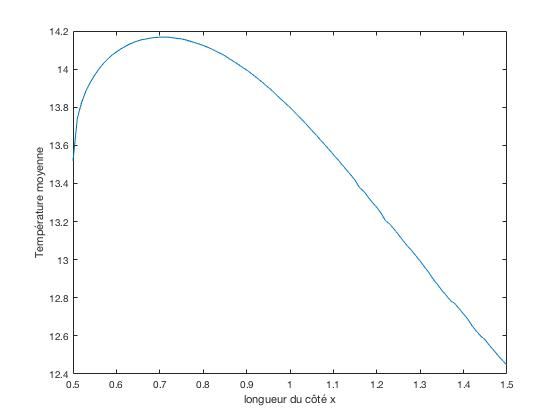
\includegraphics[scale=0.5]{Triangle_CourbeX.jpg}
\end{center}
\newpage

On trouve alors un maximum aux alentours entre $0.70$ et $0.71$ (ce qui ressemble fortement à $\frac{\sqrt{2}}{2}$). Ce n'est pas vraiment une surprise, car on s'attendait à trouver une forme relativement régulière, et dans le cas présent, il s'agit du triangle rectangle équilatéral. \\
\vspace{5cm}
\begin{center}
\begin{picture} (0,0) (20,0) 
\setlength{\unitlength}{2.5cm}
\thicklines
\put(0,0) {\line(0,1) {2}}
\put(0,0) {\line(1,1) {1}}
\put(0,2) {\line(1,-1) {1}}
\put(-0.2,1) {$1$}
\put(0.2,1) {$|\Omega|$}
\end{picture}
\end{center}
\vspace{1cm}
Procédons à quelques remarque. Tout d'abord, on observe que la figure "optimisée" est symétrique, ce qui semble s'accorder avec les conditions aux limites spatiales qui sont elles symétriques par rapport à l'axe des abscisses. Cela explique pourquoi dans la suite de l'étude, nous accorderons une place importante à la symétrie dans les figures recherchées.\\




\newpage


\newpage


\part{Déplacement d'un point du polygone à aire constante}
\section*{I - Un premier déplacement}

\pa L'idée général de l'algorithme repose sur le déplacement successif des différents points du polygone et cela en conservant l'aire totale du polygone. Pour cela on va déplacer un sommet sur la droite passant par les deux sommets voisins du sommet. Sur le schéma, nous avons représenté cette droite en rouge. L'idée derrière ce déplacement est d'exploiter la formule sur l'aire d'une triangle : $\mathcal{A} = \frac{\mathcal{B}.h}{2}$ , ou $\mathcal{B}$ est la base du triangle et $h$ est la hauteur du triangle. En déplacant les points de cette façon, nous pouvons conserver la hauteur et la base du triangle considéré par l'algorithme et par conséquent l'aire du triangle. \\

\vspace{3.5cm}
\begin{center}
\begin{picture} (100,100) (20,0) 
\setlength{\unitlength}{2.5cm}
\thinlines
\put(0,0) {\color{gray} \line(-2,3) {1}}
\put(-1,1.5) {\color{gray} \line(2,1) {1}}
\thicklines
\put(0,0){\line(-1,1){1}}
\put(-1,1){\line(1,1){1}}
\put(0,0){\line(1,0){2}}
\put(0,-0.5) {\color{red} \line(0,1) {3}}
\put(-1,-0.5) {\color{red} \line(0,1) {3}}
\put(0,2) {\line(1,0) {2}}
\put(2,2) {\line(1,-1) {1}}
\put(2,0) {\line(1,1) {1}}
\put(-1,1) {\vector(0,1) {0.48}}
\put(-1,1.5){\circle*{0.05}}
\put(-1,1){\circle*{0.05}}
\put(-1.2,1.5){$A'$}
\put(-1.2,1){$A$}
\put(0.95,1) {$\Omega$}
\end{picture}
\\
\vspace{1.5cm}
Figure : Déplacement du sommet $A$ selon l'algorithme
\end{center}
\vspace{0.5cm}
\pa L'idée est ensuite de faire varier les différents points du Polygone selon le même schéma de déplacement. Toutefois, la manière de choisir les points à déplacer et les critères d'arrêt sont encore à déterminer.
\newpage

\section*{II - Un deuxième déplacement plus souple} 
\pa L'algorithme présenté précédemment permet d'optimiser une polygone de façon relativement limitée, car les déplacements sont extrêmement spécifiques afin de conserver l'aire. Il peut alors être intéressant de chercher à trouver une méthode de déplacement des points qui permet une plus grande liberté dans le mouvement. \\

\par Contrairement à la méthode précédente, l'idée est ici de s'écarter de la notion de déplacement avec conservation de l'aire du polygone. Pour gagner en souplesse de déplacement l'idée va être d'essayer plusieurs déplacement élémentaires sur chacun des sommets amovibles pour les tester tous et trouver le meilleur déplacement. Dans l'algorithme précédente nous restions sur une droite afin de conserver l'aire du polygone, mais cette fois-ci nous allons tester des déplacements répartis sur un cercle de rayon fixé autour du point à déplacer (voir Fig.1) \\
% ---------------------- DESSIN --------------------------
\vspace{1.5cm}
\begin{center}
	\begin{picture} (150,150) (35,0) 
	\setlength{\unitlength}{2cm}

	\thicklines
	\put(0,0){\line(0, 1){2}}
	\put(0,0){\line(5,-2){2}}
	\put(0,2) {\line(5,2) {2}}
	\put(2,2.8) {\line(1,-1) {1.8}}
	\put(2,-0.8) {\line(1,1) {1.8}}
	\put(0.95,1) {\LARGE{$\Omega$}}
	\put(3.8, 1){\color{red}\circle{100}}
	\put(3.8, 1){\color{black}\circle*{0.1}}
	\put(3.9, 0.9){$A$}
	\end{picture}
	\\
	\vspace{2cm}
	Fig.1 : Zone de déplacement du sommet $A$ pour l'algorithme
\end{center}
\vspace{0.5cm}
\par Afin de discrétiser ce cercle, nous allons choisir un nombre de positions (ou directions) équitablement réparties sur le cercle. L'algorithme va ainsi pouvoir essayer toutes les configurations possibles sur le cercle afin de choisir le déplacement qui maximise la valeur moyenne. \\
\newpage
\begin{center}
	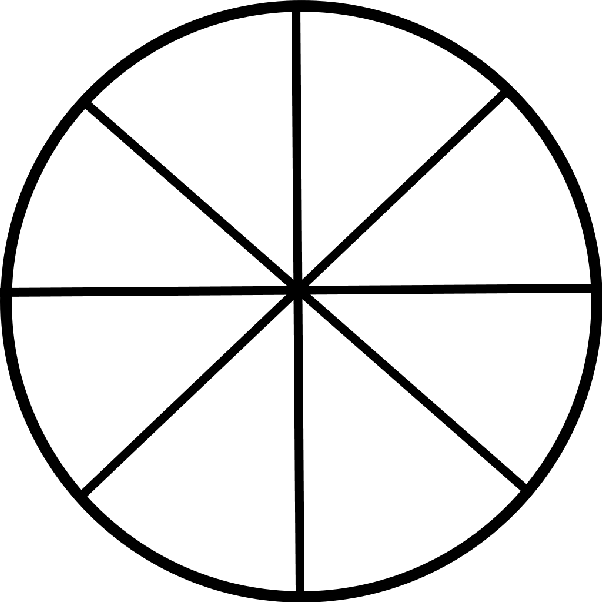
\includegraphics[scale=0.2]{positions_circle.png}\\
	\vspace{0.2cm}
	Fig.2 : Schéma dans une configuration à 8 positions
\end{center}
\vspace{0.1cm}
\par A chaque itération de l'algorithme, un déplacement va être effectué, cependant, les déplacements exposés ci-dessus ne permettent pas de conserver l'aire initiale du polygone. Nous avons donc pensé à combiner ce déplacement avec une contraction (ou décontraction) du polygone, afin qu'il possède la même aire que le polygone initial. Ainsi, nous pouvons garder la malléabilité au niveau du déplacement le tout en gardant une aire constante. La contraction du polygone est réalisée de façon assez naïve en déplaçant les points jusqu'à ce que l'on obtienne l'aire souhaitée (voir Fig.3). La contraction doit aussi obligatoirement se faire selon l'axe des abscisses car on doit absolument garder la longueur du mur modélisant le radiateur. \\

% --------------------------------------------------------

% ---------------------- DESSIN --------------------------
\begin{center}
	\begin{picture} (150,150) (35,0) 
	\setlength{\unitlength}{2cm}
	\thicklines
	\put(0, 0){\color{blue}\line(0, 1){1}}
	\put(0,1){\line(3, 1){3}}
	\put(0, 0){\line(3, -1){3}}
	\put(3, -1){\line(2, 3){1}}
	\put(3, 2){\line(2, -3){1}}
	\put(4,-1) {\LARGE{$\Omega$}}


	\put(0,1){\color{red}\line(1, 1){1}}
	\put(0, 0){\color{red}\line(1, -1){1}}
	\put(1, -1){\color{red}\line(2, 3){1}}
	\put(1, 2){\color{red}\line(2, -3){1}}
	
	% Placement des vecteurs 
	\put(3,2) {\color{red}\vector(-1,0) {2}}
	\put(3,-1) {\color{red}\vector(-1,0) {2}}
	\put(4,0.5) {\color{red}\vector(-1,0) {2}}

	\end{picture}
	\\
	\vspace{3cm}
	Fig.3 : Contraction selon l'algorithme
\end{center}


\newpage





\newpage

Regardons sur un exemple le résultat de l'algorithme

\begin{center}
	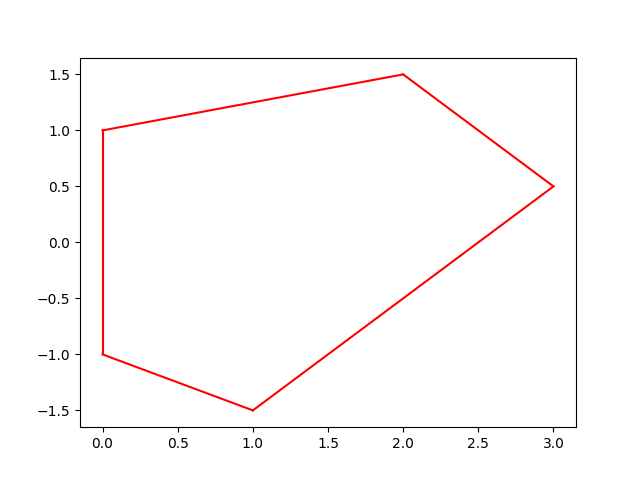
\includegraphics[scale=0.5]{initialPolygon.png}
	\\ Figure : Polygone initiale 
\end{center}

\begin{center}
	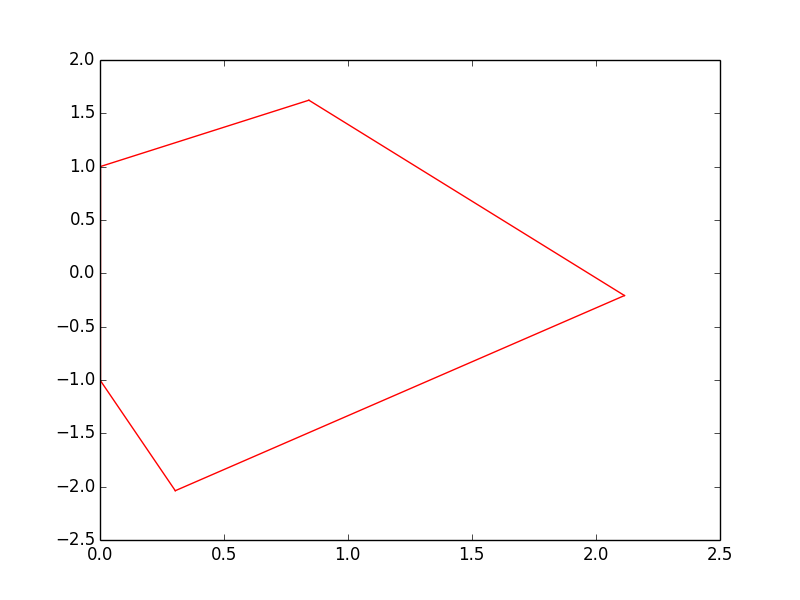
\includegraphics[scale=0.5]{finale.png}
	\\ Figure : Polygone finale, après l'algorithme 
\end{center}

Pour cet exemple comme pour les autres testés avec l'algorithme le résultat a toujours été analogue: étape après étape du processus le polygone se symétrise par rapport à l'axe de symétrie du problème (axe des abscisses, avec les valeurs choisies)

Pour les semaines à venir, nous allons essayer d'expliciter le profil des températures moyennes optimales obtenues selon les valeurs de pas utilisées en entrée de l'algorithme. Il est fort à parier qu'il soit possible de relier ce comportement à la "structure géométrique" des déplacements.
\\ Voici un premier graphique obtenu, en raison d'un nombre d'itérations trop faibles utilisé il est difficilement interprétable.
\begin{center}
	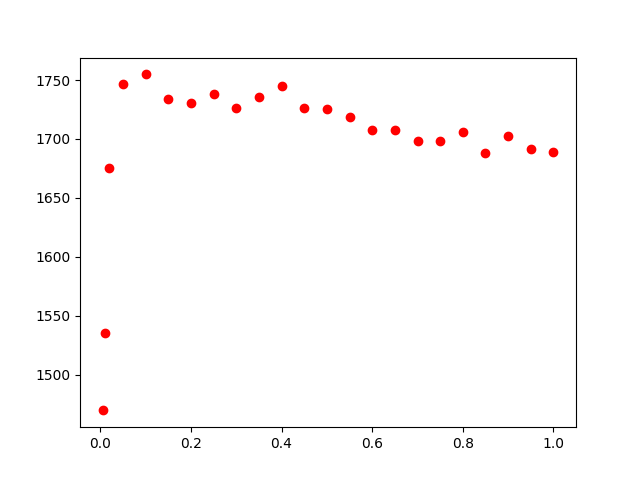
\includegraphics[scale=0.5]{plotPas.png}
	\\ Figure: valeur de la température moyenne optimale obtenue en fonction du pas utilisé pour un polygone initial donné
\end{center}


\newpage
\part{Implémentation des Algorithmes}



\section*{I - Structure générale de l'algorithme}
\pa L'algorithme implémenté est un algorithme naïf qui se contente de bouger les différents points du polygone et de trouver le meilleur déplacement pour maximiser la température moyenne à chaque itération. \\

\begin{center}
	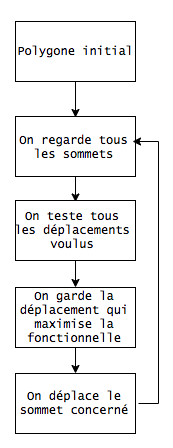
\includegraphics[scale=0.7]{algo.png}\\
	\vspace{0.2cm}
	Fig 5.1 : Schéma simple de l'algorithme d'optimisation du polygone\\
\end{center}
\vspace{0.1cm}

\section*{II - Implémentation d'un algorithme sous Python} 
\par L'idée générale est de créer un objet sous python qui représente un polygone. Nous avons opté pour la création d'une classe appelée Polygon, qui est constituée d'une liste de points indépendants, qui peuvent être bougés au gré de nos envies. 
\\
\par Tout d'abord, nous disposons, via MATLAB, d'un outil puissant et efficace de résolution des équations différentielles: la PDE toolbox. Cependant, un inconvénient de cet outil est le temps d'exécution qui est élevé. Appelons \textit{calcul\_statio} le programme qui renvoie la valeur de la température moyenne de la chambre en régime stationnaire.\\

\par Présentons schématiquement les idées générales de l'algorithme \textbf{itératif} que nous avons choisi : \vspace{0.3cm}

\begin{itemize}
	\item L'algorithme prend en entrée les coordonnées du polygone initial dans le bon ordre ainsi que le pas $p$ de déplacement;
	\item On entre dans la boucle: tous les sommets mobiles du polygones sont parcourus;
	\item Pour chaque sommet on teste les  petits déplacements stables : pour chaque déplacement on applique \textit{valueIntegral} au polygone
	\item On garde en mémoire le déplacement (éventuellement nul si pas d'amélioration) et la valeur de la température moyenne associée. 
	\item On ressort de la boucle avec le meilleur déplacement et le sommet associé
	\item On applique le déplacement au polygone, puis on recommence (il s'agit bien d'un procédé itératif). Si plus aucun déplacement ne permet d'augmenter la valeur moyenne, on arrête l'algorithme
\end{itemize}
\par En termes de représentation informatique, nous avons décidé de modéliser les polygone par une classe $Polygon$ sous Python, qui est représentée par une liste de points qui constituent les différents sommets. Ces différents points peuvent être modifiés grâce à des méthodes qui agissent sur cette instance de la classe $Polygon$. \\

\section*{III - Remarques et améliorations}

\pa Premièrement, nous pouvons remarquer que cet algorithme met en jeu une connexion entre python ou nous gérons les données relatives aux polygones et MATLAB pour faire les calculs. Cette connexion assez technique sur le plan purement informatique est couteuse en temps. Nous envisageons donc pour la suite de notre projet d'éventuellement trouver un module sur python pour y mener l'ensemble du processus. \\
\par Par ailleurs, la plus grande partie du temps d'exécution de l'algorithme a pour origine le maillage de la figure. Cette étape est essentielle pour la résolution d'une équation aux dérivées partielles. Pour optimiser notre algorithme, dans la mesure ou chaque étape n'engendre qu'une petite modification du polygone, nous pourrions éventuellement nous tourner vers des méthodes de remaillage efficaces. \\
\par Lorsque nous faisons des petits déplacements des sommets, il faut faire attention à ne pas casser "la convexité" de la figure, ce qui pourrait passer aussi par un cas singulier où notre polygone aurait un coté en moins. Nous allons ajouter un test à notre algorithme pour nous assurer qu'il n'y est pas de problème à cause de ces cas limites. \\
\par Ensuite, pour améliorer la complexité de l'algorithme, nous envisageons d'adapter la méthode du gradient et de chercher à identifier des directions privilégies.\\
\par Ensuite, une grande limitation de cet algorithme est que la valeur du pas influe grandement sur le résultat final. Contrairement à ce que nous pourrions penser naivement un pas petit n'améliore pas nécessairement la qualité du polygone finale (on peut rester bloquer sur un maximum local).\\
\par A l'heure actuelle, nous n'avons pas pris en compte les cas difficiles, et nous préférons partir de formes polygonales relativement concaves afin d'arriver à la solution sans que les déplacement ne rendent le polygone convexe. Dans certains cas, le polygone va "croiser" ses arêtes, et générer une erreur. \\
\par Les figures polygonales très dendritiques sont aussi problématiques, car la résolution de l'équation différentielle sur des zones avec un très faible angle explosent et donnent des résultats aberrants. 

\newpage

\part{Résultats des algorithmes}


\section*{I - A quoi nous attendons nous ?}

\pa A première vue il est assez difficile de prévoir la forme des polygones optimaux même si on peut éventuellement "intuiter" le résultat en espérant trouver des figures régulières (polygones réguliers). Pour se faire une vague idée des résultats, nous avons réalisé une sorte de classification des polygones, en générant une vingtaine de polygones de même aire et de les associer à une couleur proportionnelle à la valeur de leur température moyenne. Nous obtenons ainsi les résultats suivants : \\

\begin{center}
	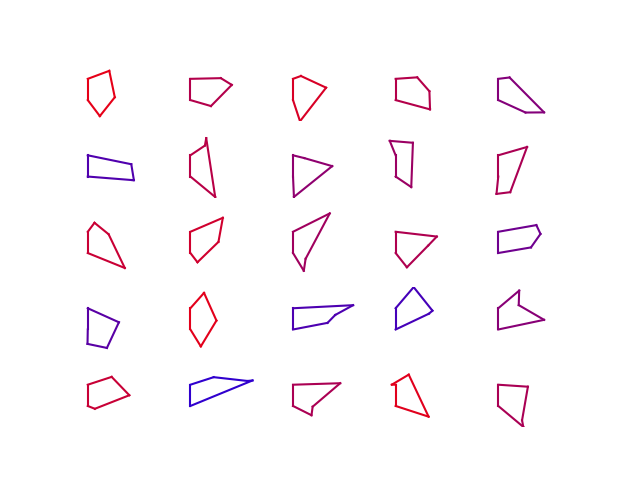
\includegraphics[scale=0.9]{Figure_3.png}
	Fig : Carte de polygones de même aire (Les polygones avec une haute valeur moyenne sont coloriés en rouge et en bleu si elle est basse)\\
\end{center}

\par De cette carte, on peut vaguement tirer quelques informations. Par exemple, il semble que les polygones "massés" autour du mur chauffé semblent posséder une meilleure valeur de température moyenne. De la même façon les figures longues, fines, assez éloignées du mur chauffé semblent posséder une valeur moyenne plus basse. Pour synthétiser cette vision, on pourrait dire que les figures les plus optimisées sont celles qui diminuent au maximum la distance de chacun des points intérieur au mur chauffé. Il semblerait aussi avec ce raisonnement que les figures symétriques soient plus optimisées.\\

\section*{II - Cas des déplacements sur les droites parallèles}

\pa Moralement on s'attend lors d'une optimisation à ce que les figures deviennent plus symétriques et tassées proche du mur. C'est effectivement ce que l'on distingue lors des simulations avec la première méthode de déplacement. Toutefois cela n'est pas frappant à cause du faible nombre d'itérations.
\begin{center}
	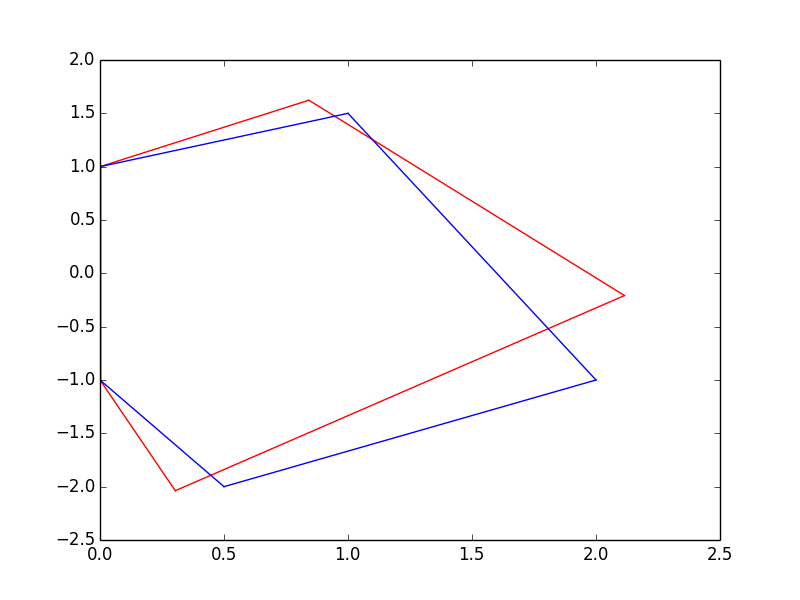
\includegraphics[scale=0.7]{test50.png}\\
	\vspace{0.2cm}
	Fig 5.1 : Optimisation d'un polygone avec la première méthode pour 50 itérations (En rouge le polygone optimisé, et en bleu le polygone initial)\\
\end{center}

\par On constate bien une amélioration globale de la température moyenne après l'optimisation, cependant ce n'est pas très satisfaisant pour deux raisons majeures : \\
\begin{itemize}
	\item L'algorithme se retrouve très vite bloqué par sa faible liberté de mouvement
	\item La forme optimisée est trop dépendante de la figure initiale choisie, et dépend énormément du pas de déplacement choisi
\end{itemize}

\par Ce sont en partie ces constats qui nous ont poussé à chercher d'autres méthodes de déplacement des points, afin de gagner une plus grande liberté en terme de déplacement.\\
\newpage 

\section*{III - Cas des déplacements améliorés}

\pa La plus grande liberté de mouvement donnée par la méthode utilisée nous laisse espérer que les solutions données par cet algorithme seront meilleures que celles données par l'algorithme précédent. Afin de constater cela, nous allons réaliser une comparaison sur deux exemples de polygone différents, mais de même aire pour 50 itérations :  \\

\begin{center}

	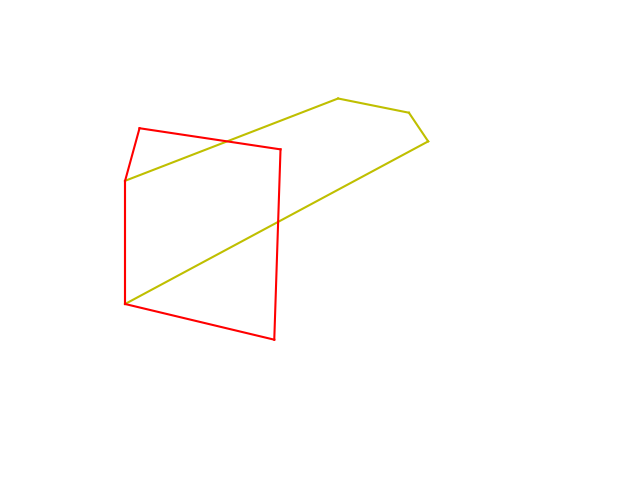
\includegraphics[scale=0.45]{resultat_souple_2.png}
	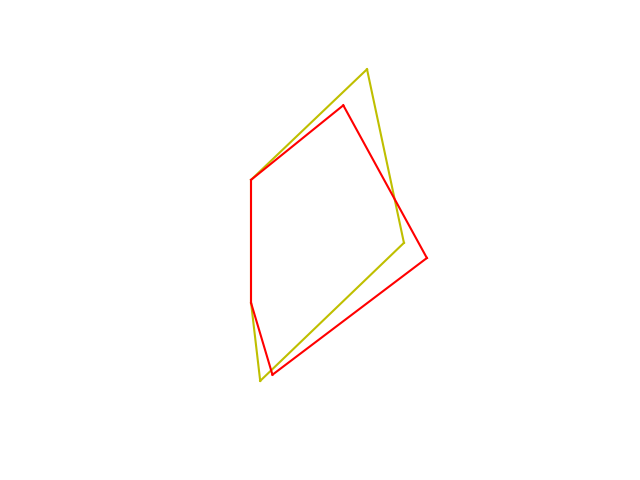
\includegraphics[scale=0.45]{resultat_souple_4.png}\\
	Fig : En jaune le polygone initial, et en rouge le polygone optimisé (voir Annexe pour les détails)
\end{center}

\vspace{2cm}

\par La conjecture émise dans la première section semble bien s'appliquer au vue de la première optimisation présentée ci-dessus. La deuxième est effectivement moins flagrante. \\ 

\par Il est cependant assez difficile de comparer les deux méthodes sérieusement à partir de quelques observations. Nous avons donc réalisé quelques comparaisons sur des polygones, mais étant donné le temps de simulation, nous avons du nous contenter d'une dizaine de comparaisons. \\

\newpage
\begin{center}
	\textit{20 itérations}\\
	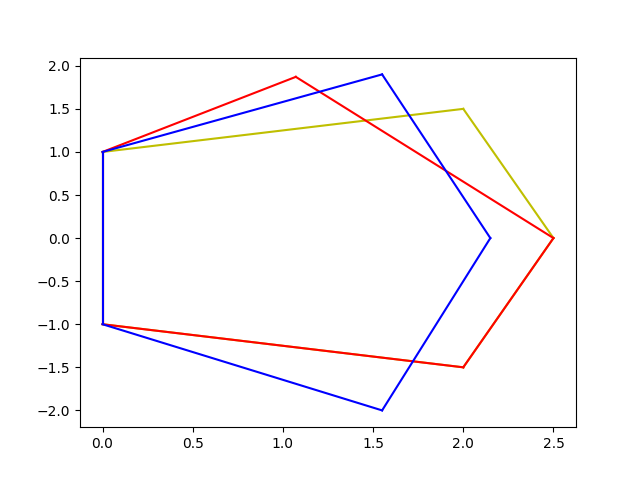
\includegraphics[scale=0.45]{comp1.png}\\
	\textit{50 itérations}\\
	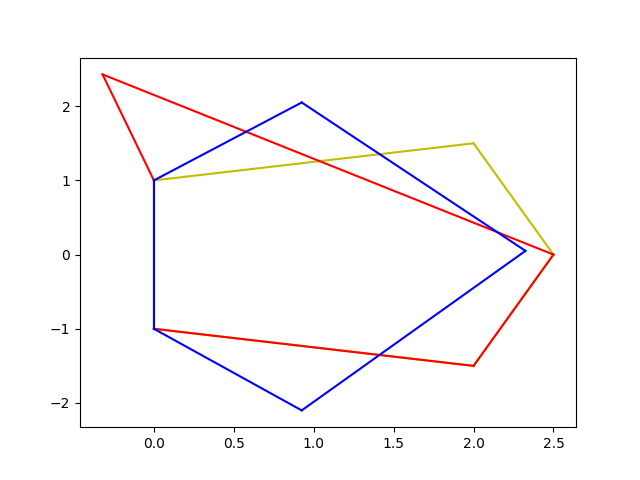
\includegraphics[scale=0.45]{comp2.png}\\
	Fig : En jaune le polygone initial, et en rouge le polygone optimisé avec la méthode 1, et en bleu avec la méthode 2
\end{center}

\par On constate clairement une nette avance de la seconde méthode. La méthode 1 étant très limitée en terme de liberté de mouvement, elle n'a pas permis d'optimiser correctement la figure montrée dans la simulation ci-dessus. \\ 

\par Cet algorithme semble bien plus satisfaisant que le premier dans la mesure ou pour un même nombre d'itérations la figure est largement plus optimisée.



\section*{IV - Exploitation des symétries}

\pa Comme l'on s'attend plutôt a ce que les figures optimales soient symétriques, il peut être intéressant de partir de figures déjà symétriques et d'exploiter la symétrie du polygone pour le déplacer avec la méthode de nôtre choix, mais en conservant la symétrie. Les avantages sont multiples si l'on tient compte de cela. Tout d'abord, on réduit par 2 le nombre de calculs de température moyenne ce qui diminue drastiquement le temps de simulation. D'autre part, il y a une plus rapide convergence de l'algorithme vers un polygone optimal lorsque l'on tient compte des symétrie. \\ 

\par En reprenant le polygone de l'exemple précédent, et en appliquant une fois l'algorithme basique et une fois en exploitant les symétries avec les mêmes paramètres, on obtient les résultat suivants : \\ 

\begin{center}
	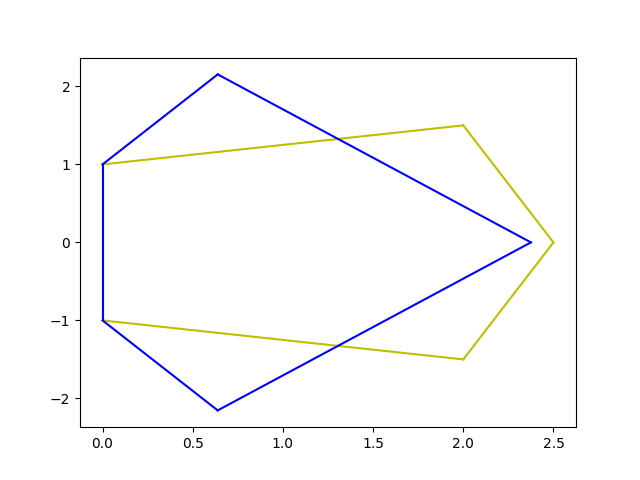
\includegraphics[scale=0.45]{symetrieAlgo.png}\\
	Fig : Exploitation des symétries (18 itérations, Valeur : 1763)\\
	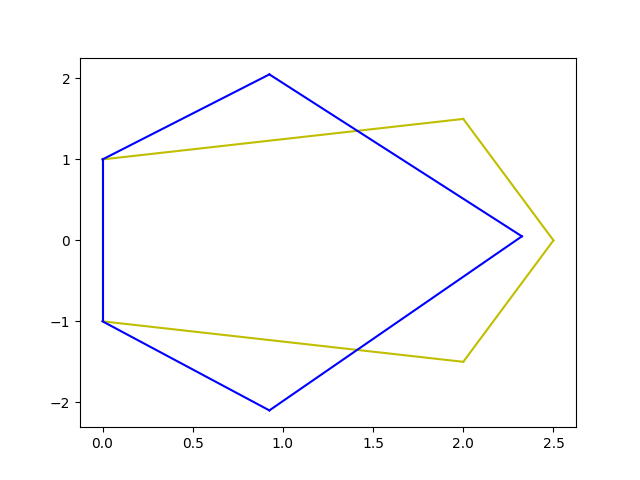
\includegraphics[scale=0.45]{comp3.png}\\
	Fig : Non Exploitation des symétries (49 itérations, Valeur : 1733)

\end{center}












% --------------------------------------------------------
\newpage





% ///////////////////////////////////////////////////////
%						        Partie Annexes
% ///////////////////////////////////////////////////////

\part*{Annexes}

%========================================
% Classe VECTOR
%========================================

\section*{Classe Vector}

Cette première classe permet juste de représenter des vecteurs dynamiques sous Python.


\begin{lstlisting}[language=Python,frame=single,caption=Création de la classe Vecteur]
class Vector : 
    """ Represente un vecteur """
    
    def __init__(self,x,y) : 
        self.x = x 
        self.y = y 
        
    def __str__(self) : 
        return ("v(%f,%f)" % ( self.x, self.y))
        
        
    # Normalise le vecteur 
    def normalize(self) : 
        norm = (self.x ** 2 + self.y ** 2) ** 0.5
        self.x = self.x / norm 
        self.y = self.y / norm 
\end{lstlisting}


%========================================
% Classe VERTEX
%========================================

\section*{Classe Vertex}

La classe Vertex permet de représenter des sommets mobiles sous Python. Chaque polygone est ainsi constitué de plusieurs objets de classe Vertex (de plusieurs sommets). La classe contient notamment une fonction $move$ permettant de déplacer un point selon une droite.

\begin{lstlisting}[language=Python,frame=single,caption=Création d'une classe Vertex]
class Vertex : 
    """
     La classe Vertex est une classe qui represente les coordonnees des points 
     d'un polygone donne 
    """
    
    def __init__(self, x, y) : 
        
        self.x = x 
        self.y = y 
    
    def __str__(self) : 
        return ("(%f,%f)" % (self.x, self.y) )
    
    def __copy__(self, vertex) : 
        self.x = vertex.x 
        self.y = vertex.y 
    
    #---------------------------------------------------------------------    
    # Deplace le sommet de dx selon x et dy selon y 
    
    def update(self, dx, dy) : 
        self.x += dx 
        self.y += dy 
        
        
    #---------------------------------------------------------------------   
    # deplace le point dans la direction du vecteur unitaire vector 
    
    def move(self, vector, dl) : 
        # On deplace le point selon le vecteur
        dx = dl * vector.x 
        dy = dl * vector.y 
        self.update(dx, dy) 
\end{lstlisting}

%========================================
% Classe POLYGON
%========================================

\section*{Classe Polygon}

La classe Polygon est l'élément central de notre optimisation de forme. En effet nous cherchons à optimiser des objets de forme polygonale. \\
Chaque objet Polygon est constitué d'objets de classe Vertex qui contiennent les coordonnées des sommets. Ces Vertex sont contenus dans un attribut de type liste, et ils sont ordonnés dans le sens horaire. On commence conventionnellement par mettre les sommets liant le côté traversé par le flux. C'est très important, car le calcul de la température moyenne sous Matlab dépend de l'ordre des côtés, car il faut choisir des conditions aux limites différentes sur chacun des côtés.\\
Les méthodes de cette classe Polygon sont les suivantes : 
\begin{enumerate}
\item $init$ qui initialise la classe avec une liste \textbf{ordonnée} de sommets de type Vertex
\item $deepCopy()$ qui permet de copier un objet
\item $getx(i)$ et $gety(i)$ qui retournent les coordonnées $x$ et $y$ du sommet numéroté i 
\item $directorVertice(i)$ qui retourne le coefficient directeur de la droite passant par le sommet i, et parallèle à ses deux voisins les plus proches (voir la droite rouge sur le schéma du déplacement)
\item $directorSide(i)$ qui retourne le coefficient directeur de la droite passant par le côté numéroté i 
\item $buildGeometry()$ qui construit une liste représentant le polygone en Matlab. Cette liste est exportée sous Matlab pour être traitée. 
\item $move(i, dl)$ qui bouge le sommet numéroté i d'une distance dl \textbf(Attention : dl peut être négatif)
\item $valueIntegral(i, dl, eng)$ qui calcule la température moyenne dans le polygone lorsque le sommet i est déplacé d'une longueur dl. Cette fonction est déclinée en $valueIntegralOS(i, dl, eng)$ (OS:odd sides and symetrical) qui prend en compte la symétrie dans le mouvement
\item $plotPY(color)$ qui trace sur le canvas le polygon (pour faire des représentations graphiques
\item $area()$ qui calcule l'aire du polygone grâce à un module spécifique
\item $degSymetrie()$ qui calcule le "degré de symétrie" du polygone grâce à un module encore une fois 
\
\end{enumerate}
\newpage


\begin{lstlisting}[language=Python,frame=single,caption=Création de la classe Polygon]

class Polygon :

    """
        La classe Polygon contient des Vertex (Sommets). L'ensemble de ces sommets
        forme un polygon

        Les attributs de cette classe sont :
           N : le nombre de côtés
           vertices : la liste contenant les sommets

    """

    def __init__(self, *args) :
        # Nombre de côtés dans le polygone
        self.N = len(args)

        # Liste contenant les sommets (vertex)
        self.vertices = []
        for vertex in args :
            self.vertices.append(vertex)

    def deepCopy(self):
        copy = Polygon()
        copy.N = self.N
        for vertex in self.vertices :
            copy.vertices.append(vertex.deepCopy())
        return copy


    # Print
    def __str__(self) :
        res = "("
        for vertex in self.vertices :
            res = res + vertex.__str__() + ","
        return res[:-1]+')'


    #----------------------------------------------------------------
    # Retourne les coordonnées x et y d'un sommet
    #
    # Retourne la coordonnée x du sommet i
    def getx(self, i) :
        return self.vertices[i % self.N].x

    # Retourne la coordonnée y du sommet i
    def gety(self, i) :
        return self.vertices[i % self.N].y



    #-----------------------------------------------------------------
    # La fonction findCoef renvoie le coefficient directeur de la droite passant
    # par les sommets i-1 et i+1

    def directorVertice(self, i) :
        dx = self.getx(i + 1) - self.getx(i - 1)
        dy = self.gety(i + 1) - self.gety(i - 1)
        res = Vector(dx, dy)
        res.normalize()
        return res



    #-----------------------------------------------------------------
    # calcule le vecteur directeur de la droite passant par le côté i
    def directorSide(self, i) :
        dy = self.gety(i + 1) - self.gety(i)
        dx = self.getx(i + 1) - self.getx(i)
        res = Vector(dx, dy)
        res.normalize()
        return res


    #-----------------------------------------------------------------
    # Cette méthode construit une géométrie prête à l'exportation sous matlab

    def buildGeometry(self) :

        #    On initialise une liste avec l'argument 2, qui est le 
        #    code correspondant a une forme polygonale sous 
        #    matlab, et self._N est le nombre de côtés
 		#    Cette fonction renvoie une matrice prête a être 
 		#    employée dans la fonction Matlab decsg(mat)

        mat = [[2], [self.N]]
        for vertex in self.vertices :
            mat.append([vertex.x])
        for vertex in self.vertices :
            mat.append([vertex.y])
        return mat

    #-----------------------------------------------------------------
    #
    #    Déplacement d'un point du polygone selon l'algorithme
    #    i correspond au numéro du sommet et dl à la longueur du déplacement

    def move(self, i, dl) :
        vector = self.directorVertice(i)
        self.vertices[i % self.N].move(vector, dl)


    #------------------------------------------------------------------
    #
    #    Calcul de la valeur de l'intégrale pour un déplacement
    #    du sommet i d'une longueur dl. La méthode ne modifie ainsi
    #    pas le polygone lorsque elle est executée

    def valueIntegral(self, i, dl, eng) :
        self.move(i, dl)
        mat = matlab.double(self.buildGeometry())
        value = eng.computeIntegral(mat)
        self.move(i, -dl)
        return value

    #-------------------------------------------------------------------
    #
    #   La fontion calcul calcul aussi l'intégrale, mais pour un
    #   un déplacement symétrique du polygone symétrique à côtés
    #   impairs (On exploite donc la symétrie)

    def valueIntegralOS(self, i, dl, eng) :
        self.move(i, dl)
        self.move(self.N - i, -dl)
        mat = matlab.double(self.buildGeometry())
        value = eng.computeIntegral(mat)
        self.move(i, -dl)
        self.move(self.N - i + 1, dl)
        return value


    #--------------------------------------------------------------------
    # Fonction de traçage

    def plotPY(self,color) :

        for k in range(self.N) :
            plt.plot([self.vertices[ k % self.N].x,
                      self.vertices[(k + 1) % self.N].x],
                     [self.vertices[k % self.N].y,
                      self.vertices[(k + 1) % self.N].y],
                     color
                     )

        #plt.show()


    #---------------------------------------------------------------------
    # Retourne l'air du polygone

    def area(self) :

        poly = [[self.getx(i), self.gety(i)] for i in range(self.N)]
        return aire_poly(poly)

    #---------------------------------------------------------------------
    # Retourne l'air du polygone

    def degSymetrie(self, step) :

        poly = [[self.getx(i), self.gety(i)] for i in range(self.N)]
        return deg_sym(poly, step)


\end{lstlisting}


%========================================
% SCRIPT PRINCIPAL MATLAB
%========================================
\section*{Calcul de la valeur moyenne sous Matlab}

Le script suivant est une fonction prenant en argument une forme géométrique sur laquelle va être résolue l'EDP. Voici le fonctionnement de la fonction résumée :

\begin{enumerate}
\item La géométrie importée est implantée dans l'objet model qui va servir à résoudre l'équation differentielle
\item avec $applyBoundaryCondition$ on applique les conditions aux limites sur le modèle étudié (ici dirichlet sur tous les côtés sauf le premier avec une valeur 10, et newmann sur le premier côté avec une valeur 10000
\item Ensuite on résout l'équation de la chaleur (f=0 car pas de termes de source). Les variables u, p, t contiennent respectivement les valeurs scalaires de la fonction, les coordonnées des sommets, et les références de chaque sommets
\item A l'aide de ces dernières variables, on calcule l'intégrale de la fonction solution (C'est à dire la température moyenne)
\end{enumerate}



\begin{lstlisting}[language=Matlab,frame=single,caption=Script Matlab pour le calcul de la valeur moyenne sur une géométrie donnée]

function I = computeIntegral(mat) 


model = createpde() ; 
g=decsg(mat);
geometryFromEdges(model,g); % geometryFromEdges for 2-D


edges = [2:1:(size(mat)-1)/2];
%Conditions de bord : 
%Les murs non chauffés sont  la température éxterieure To = 10C
applyBoundaryCondition(model,'dirichlet','Edge',edges,'u',10);

%Le mur chauffé est modelisé par un flux rentrant , on suppose que l'on a
%mis un radiateur au niveau du mur 
applyBoundaryCondition(model,'neumann','Edge',[1],'q',0,'g',10000);

a = 0;
c=1;
a=0;
f=0;
[u,p,e,t] = adaptmesh(g,model,c,a,f,'Par',0.1,'tripick','pdeadworst',
	               'MesherVersion','R2013a');



%Le résultat est ainsi renvoyé
%On calcule l'intégrale de la fonction renvoyée

coord = p ; % Contient les coordonnées des sommets 
indices = t ; % Contient les références de chaque élément
val = u ; 

% On va calculer l'intégrale en évaluant la valeur de la fonction sur
% chaque petit triangle 

I =0 ; 
area = 0 ; 
for i = 1:length(indices) ; % Pour chaque triangle 
    a = coord(:,indices(1,i)) ;     % Coord du 1er point 
    b = coord(:,indices(2,i)) ;     % Coord du second point 
    c = coord(:,indices(3,i)) ;     % Coorddu troisième point
    
    moy = (val(indices(1,i))+val(indices(1,i))+val(indices(1,i)))/3 ;
    area = area + 0.5 * abs( a(1) * c(2 )- a(1) * b(2) + b(1) * a(2) - b(1) * 
    c(2) + c(1) * b(2) - c(1) * a(2)) ; 
    I = I + moy * 0.5 * abs( a(1) * c(2) - a(1) * b(2) + b(1) * a(2) - b(1) * 
    c(2) + c(1) * b(2) - c(1) * a(2)) ;
end
    I = I / area ; 

\end{lstlisting}

%========================================
% MEILLEUR DEPLACEMENT
%========================================

\section*{Implementation de l'algorithme d'optimisation sous Python}

On commence tout d'abord par créer une fonction $bestValue$ qui prend en argument un polygone, la valeur de l'intégrale sur ce polygone (pour un soucis d'optimisation de temps de calcul), le numéro du sommet que l'on veut étudier (i), le nombre de test que l'on veut effectuer de part et d'autre du sommet (nbTest), la taille du déplacement (dl) et le moteur matlab (eng)\\
Cette fonction renvoie la valeur maximal, et le déplacement associé à cette valeur maximale dans une liste. Cette liste est de la forme [Valeur Maximale, déplacement associé (scalaire algébrique)]
\newpage
\begin{lstlisting}[language=Python,frame=single,caption=Fonction permettant de trouver la meilleure valeur de la temperature pour le déplacement d'un seul sommet]

# =============================================================================
#                             Best Value of a vertex
# =============================================================================

#   On cherche la position du sommet i qui maximise la fonctionnelle de forme
#   la fonction prend en paramètres :
#
#   - initValue : la valeur de l'intégrale du polygone initial (pour optimiser
#     et ne pas avoir à le calculer à chaque fois)
#
#   - dl : la longueur du pas
#
#   - i : le numéro du sommet
#
#   - nbTest : le nombre de valeur testée de part et d'autre du sommet, en tout
#     2*nbTest valeurs sont testées sur chaque sommet
#
#   - eng : le moteur matlab
#

def bestValue(polygon, initValue, i, nbTest, dl, eng) :

    #   On stocke les valeurs des intégrales liées à chacun des déplacements
    #   dans une liste
    #   right correspond aux déplacements à droite du point
    #   left correspond aux déplacement à gauche du point

    left = [polygon.valueIntegral(i, -j * dl, eng) for j in range(nbTest)]
    right = [polygon.valueIntegral(i, j * dl, eng) for j in range(nbTest)]
    L = np.array(left + [initValue] + right)

    #   On cherche le maximum dans cette liste, puis on trouve l'index de ce
    #   maximum, qu'on appelle indexMax
    indexMax = np.argmax(L)

    #   Le résulat retourné contient la valeur maximum de l'intégrale,
    #   et le déplacement associé à celui-ci
    return [L[indexMax], (indexMax - nbTest) * dl]


\end{lstlisting}

\vspace{3cm}
Désormais, on peut écrire la boucle principale de l'algorithme. Comme il s'agit de la première version, nous l'appelons $naiveMainloop$ car elle n'est pas très optimisée. \\
Les arguments pris en compte sont : 
\begin{enumerate}
\item La forme initiale polygon
\item la taille du pas de déplacement dl 
\item le nombre de tests (nbTest) à effectuer sur chaque déplacement
\item le nombre d'itérations maximal (nbIteration)
\item une liste values pour stocker les valeurs de la température moyenne lors de chaque itération
\item l'instance de matlab en cours (eng)
\end{enumerate}

Le principe de fonctionnement est tel qu'il est énoncé dans la description initiale de l'algorithme. On parcourt tous les sommets, et on retient seulement un seul déplacement de sommet qui maximise la température moyenne.
\begin{lstlisting}[language=Python,frame=single,caption=Boucle Principale]

# ============================================================================
#                              Naive Mainloop
# ============================================================================

#   Cette boucle naive se contente de parcourir les sommets pour trouver le
#   meilleur déplacement possible


def naiveMainloop(polygon, dl, nbTest, nbIteration, values, eng) :
    #   Conservation des données de la temperature moyenne pour chaque itération
    #   values est une liste vide destinée à conserver les valeurs de l'intégrale

    if nbIteration == 0 :
        print("Fin de la simulation")
        return 0

    initValue = polygon.valueIntegral(0,0,eng)

    #   On cherche le petit déplacement qui maximise notre fonctionnelle
    #   de forme lors d'une itération de l'algorithme
    #   On examine chacun des sommets indépendamment

    max = [0,0]                            # Initialisation du maximum
    rank = 0
    for i in range(2, polygon.N) :
        val = bestValue(polygon, initValue, i, nbTest, dl, eng)
        if val[0] > max[0] :
            max = val
            rank = i

    #   Si la valeur maximum est atteinte pour un déplacement nul,
    #   on arrête la simulation
    if max[1] == 0 :
        print("Il reste " + str(nbIteration) + " itérations")
        return 0

    # Sinon on bouge un sommet
    polygon.move(rank, max[1])
    values.append(max[0])

    # Appel récursive de la fonction
    naiveMainloop(polygon, dl, nbTest, nbIteration - 1, values, eng)
    
\end{lstlisting}

\newpage
\section*{Modules complémentaires}

\end{document}
